\chapter{Introduction}

The goal set forth by this thesis seems ambitious: to introduce a completely new language of uncertainty and information that abstracts away measure theory, probability, etc. and is better primed for computation in estimation and stochastic control algorithms.
Luckily, much of this language was already developed by much smarter people than the author. This thesis simply presents the language to a certain audience in a slightly more approachable manner, and frames it in the context of engineering problems.

Here, we also explicitly formulate certain problems such as estimation filters and stochastic control in this language.

This report is more philosophical in nature, and errs on the side of arguing for a change in pedagogy.
This report is definitely more ``big picture'', and does not dive into much of the finer nuances of control and estimation. (** E.B. no need to be so apologetic. Say what you want to say but do not ``encourage'' the reader to view this work as philosophical rather than technical **.\todo{write this better}

\todo{expand the introduction.}

\chapter{Motivation}

Deriving new estimation algorithms is hard. ** E.B. Why is hard? Explain to me the key challenges** 
This methodology (** which methodology? **) distills the complex bits into elemental building blocks.

\todo[inline]{Make a list with a breakdown of the Markov category axiom methods}

\section{Assumptions Made in the Kalman Filter}
** Do you want to devote a whole section on the assumptions of KF or present it quickly (in  a way that will facilitate the subsequent discussion) together with each assumptions? ** 

\section{Abstract Programming}

\begin{figure}[htb]
    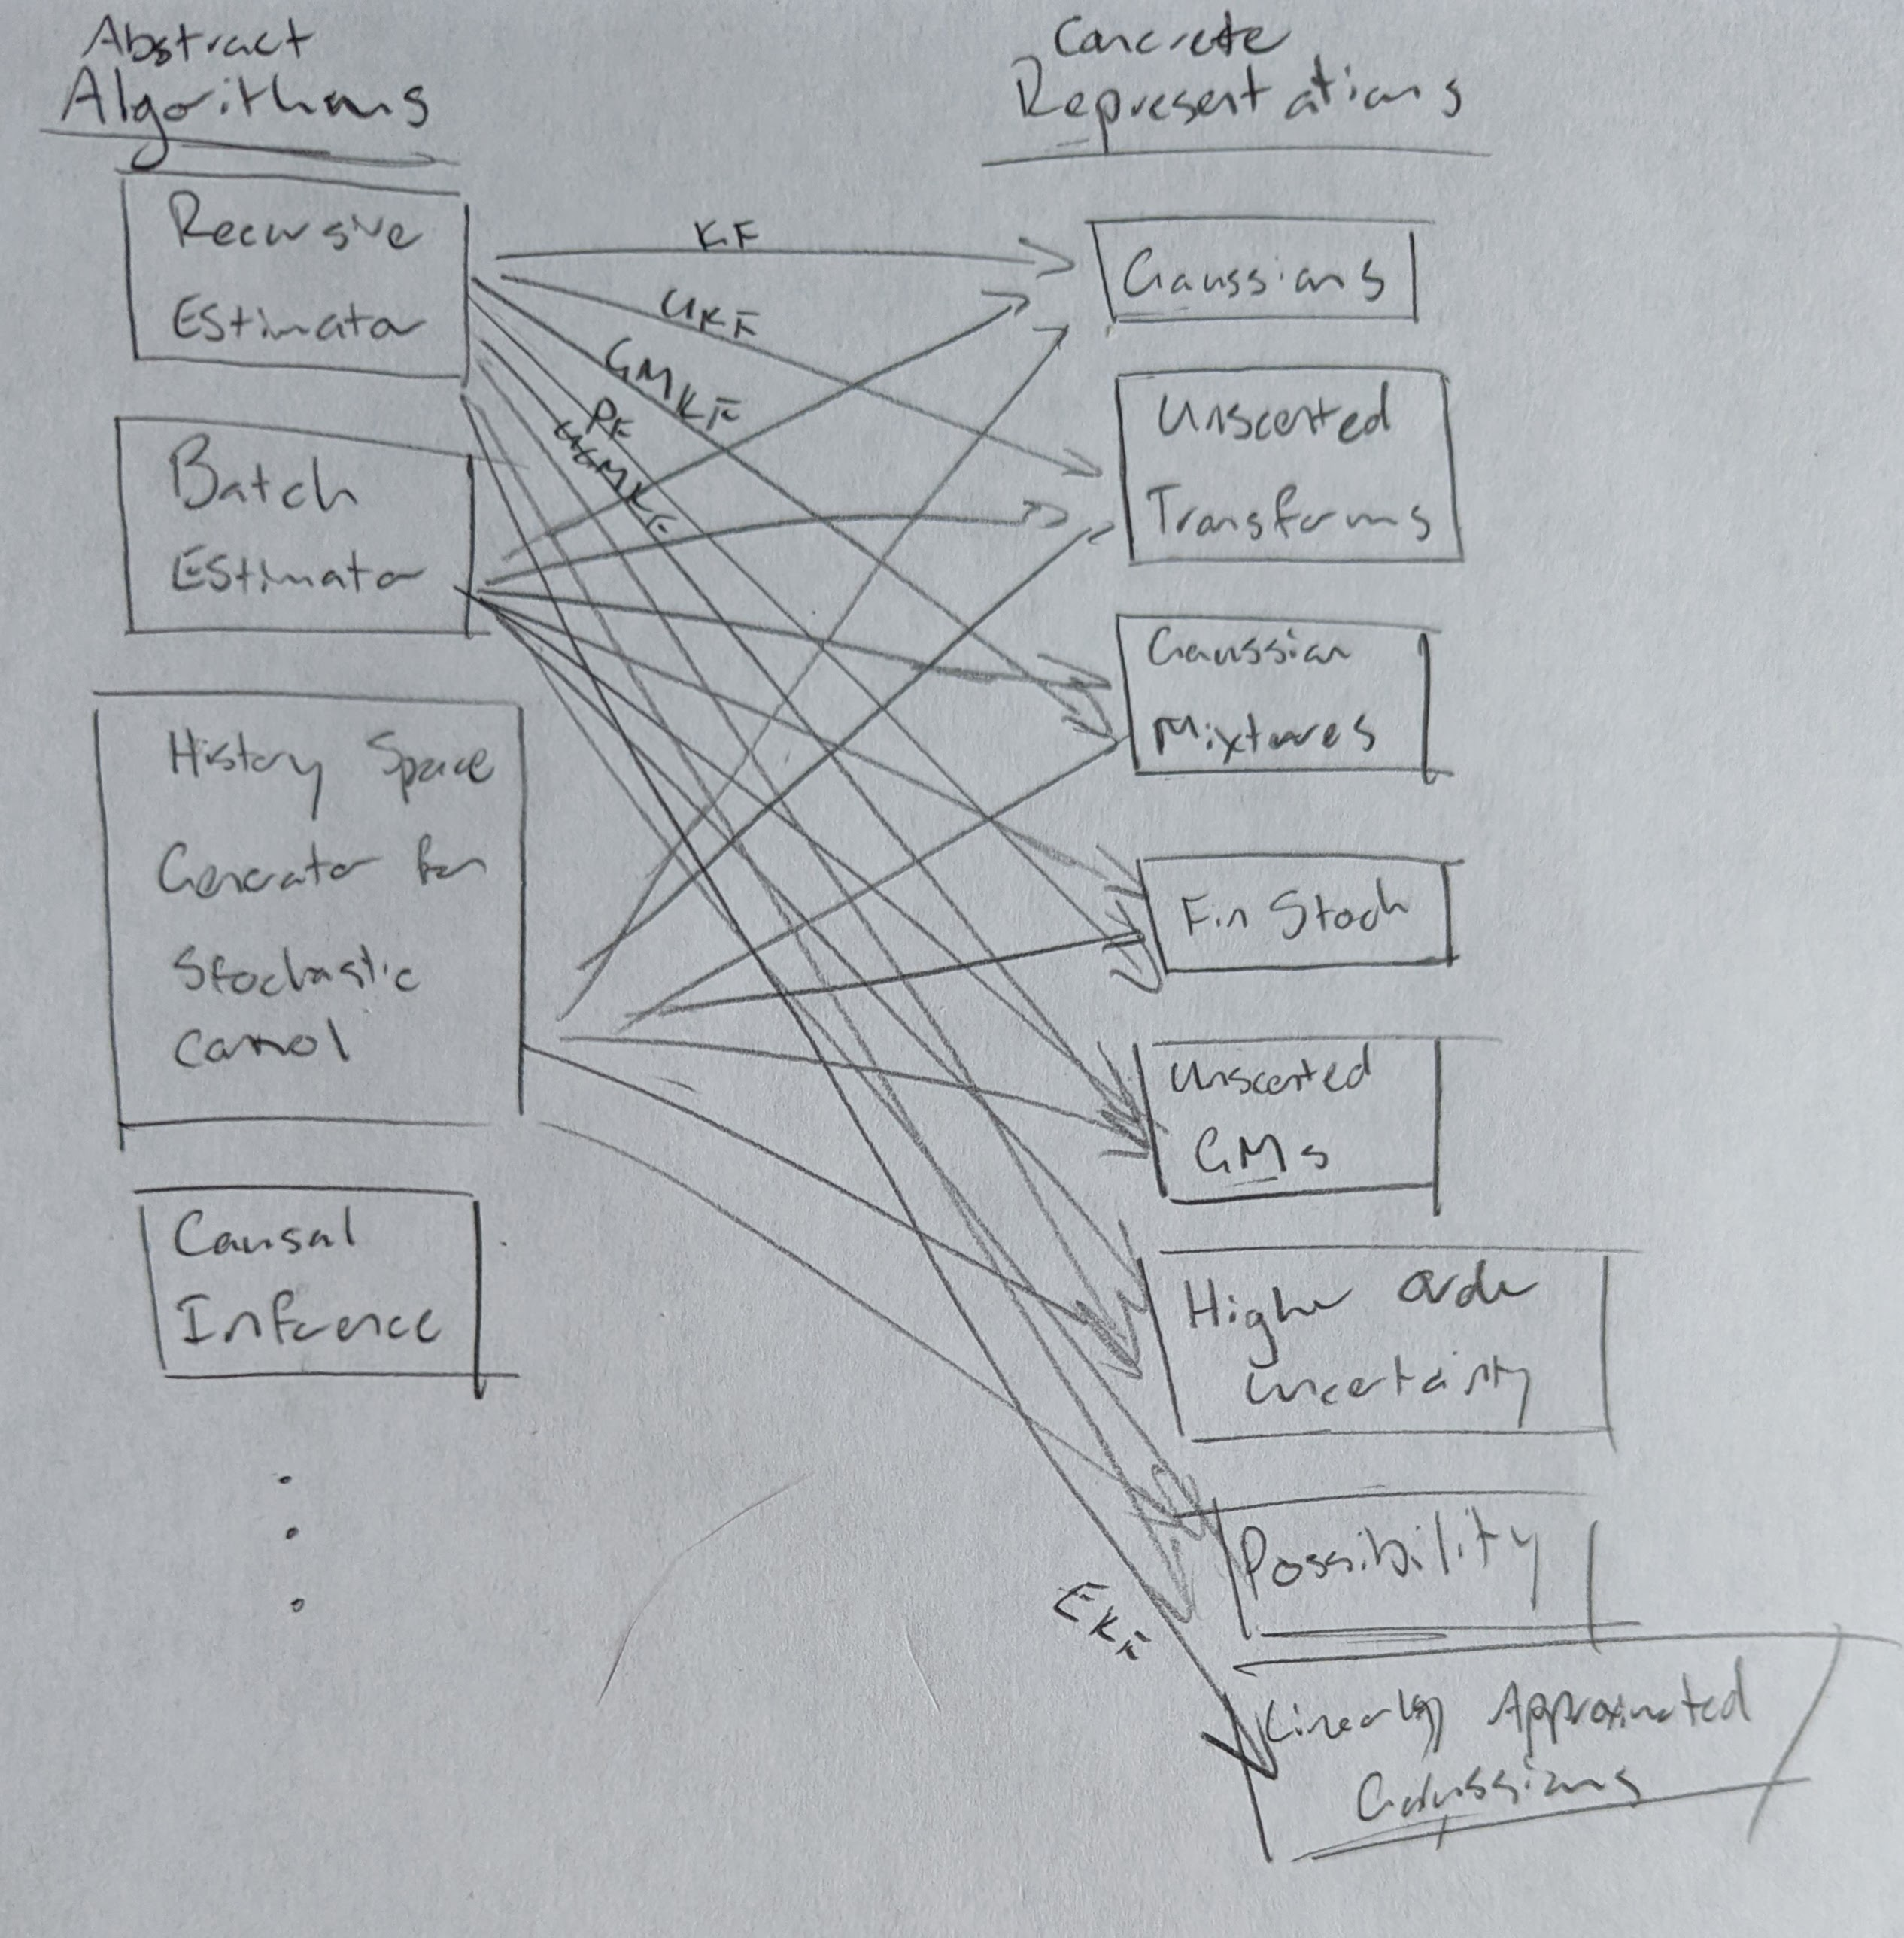
\includegraphics[width=0.5\textwidth]{algorithm-inheritance}
	\caption{}
    \label{fig:algorithm-inheritance}
\end{figure}

\chapter{Looking at Markov Transition Kernels}

There is often some conflation between conditionals and transition kernels.
In a way, they are often considered to be developments from the basics of probability.
This stems from the fact that in traditional probability theory, the probability distribution or probability measure is the fundamental notion from which all other definitions and developments are derived.
Similar to how in categorical thinking, where the perspective is switched from sets being fundamental to functions being fundamental, we want to change lenses away from distributions and onto kernels as being the most elemental construction from which distributions, statistics, and algorithms are derived. 
Of course, it significantly helps us in our understanding if we already have some insight into a traditional measure-theoretic way of thinking about probability, but this is not totally necessary.
It more serves as a grounding point, similar to when learning category theory -- it helps greatly to already be familiar with sets+functions, vector spaces+linear maps, topoligical spaces+continuous maps, groups+group homomorphisms, and so on so that we have a \emph{context} for where categories are really useful as a language to describe stuff instead of only this abstract notion of arrows and objects and categories of categories.

Before giving a formal definition of categories, we should just mention for the familiarity of the reader that a category is made of arrows called \emph{morphisms} that are useful in describing mappings between spaces. In categorical probability, these morphisms can describe \emph{mappings that behave like Markov transition kernels}.

But what exactly is a transition kernel?
Intuition would say that it is a mapping between distributions, but there is a bit more nuance than that.

\newcommand{\normal}{\mathcal{N}}
\newcommand{\reals}{\mathds{R}}
\begin{equation}
\label{traditional-gaussian-model}
\begin{gathered}
    y = Fx + w \\
    w \sim \normal(\bar{w}, R)
\end{gathered}
\end{equation}

\begin{equation}
    \begin{aligned}
	y = f(x,w)
    \end{aligned}
\end{equation}
\todo{Talk about how this has randomness pushback}
\todo[inline]{Talk about how the frequentist view of these kernels sees that w gets sampled in the instant that y gets evaluated, and acts as a modifier to Fx. We want to change this to a Bayesian view, where F evaluates by taking in an x and returning a distribution. A p(y|x) kind of thing. The problem is that bar notation, tilde notation, and distributions in the Bayesian context SUCK. This is where the functors come in.}

\todo{List a bunch of variations on kernels, and discuss them.}

One minor change to our language that can have significant impact is in the recasting of equations into functions\todo{expand on this}.

\section{Recasting the Datatypes}
The trouble with random variables:
Random variables suck. Here's why...

Random variables are often pitched to the student as variables that take on values (ie.\ real numbers) in a random fashion.
There is a frequentist sort of nature to this description, as if a random variable is a number that changes its value every time you look at it.

There is an alternative viewpoint: what is often called the Bayesian view of probability.
It states that probability (of an event) is simply a measure of our belief in a state, or more specifically the amount we believe that a state will fall into that event.
We wish to take this viewpoint and run with it, generalizing into many different ways of characterizing our belief or information on the state of a system.

\newcommand{\gaussian}{\mathcal{N}}
\newcommand{\gausscat}{\mathrm{Gauss}}
Given a real finite dimensional vector space $X$, we will define for now\footnote{This and the treatment in \ref{sec:kernel-signature} looks like we're setting up $\gaussian$ as a functor for formulating $\gausscat$ as a Kleisli category. It's well conjectured that $\gausscat$ is not a Kleisli category. For demonstration purposes however, I'm setting it up like one here to introduce readers to the concept using familiar constructions. We will discuss decorated maps a-l\`a \cite{stein2022extended} later.} the collection of Gaussian distributions on $X$.
For the practical purposes of making datatypes, it's sufficient to define it through its parameterization of a mean and covariance as opposed to defining it as the actual collection of Gaussian probability measures.
Thus, we define $\gaussian$ as a type-level\footnote{Defined later in our discussion of functional programming} mapping on vector spaces:

\newcommand{\symmetric}{\mathds{S}}
\begin{equation}
    \gaussian : X \mapsto \{(x,P) : x\in X, P \in \symmetric^X_+\}
\end{equation}

\section{The Signature of Kernels}
\label{sec:kernel-signature}

One confusing aspect of Markov transition kernels is their signature. 
Standard texts describe the a kernel as the following:

\todo{markov kernel definition}

The important bit is in the partial application: parameterizing $\kappa$ with $x$, the function $\kappa(\cdot, x)$ is a probability measure from $\mathcal{B} \rightarrow [0,1]$ and parameterizing with $B\in \mathcal{B}$, the function $\kappa(B,\cdot)$ is a \emph{mapping whose domain is $X$}.
This is important: $\kappa$ does not input values of distributions, but rather values of state.
This is evident in the confusing bar notation: $p(y|x)$ reads as ``$p$ of $y$ given $x$".
In other words, the transition kernel gives a distribution on $Y$ given a fixed value of $x\in X$.

\newcommand{\giry}{\mathcal{P}}
Using Currying ie.\ partial application\todo{expand on this?}, we can rewrite this signature. 
Since $\giry Y$ is defined to be the collection of distributions on $Y$, then there is an equivalence between $\kappa : \mathcal{B} \times X \rightarrow [0,1]$ and $\kappa : X \rightarrow \giry Y$.

We can give the same treatment to Gaussian models of the form in Equation \ref{eq:traditional-gaussian-model} in Kalman filters, which are also just Markov kernels. The maps just happen to be linear and the distributions gaussian.
While we treat $x$ as a random variable in $y = Fx + w$, the $F$ does not take in random variables.
It takes plain old vectors.
We had to do the work of figuring out how to propagate covariance through $F$.
Further, \ref{eq:traditional-gaussian-model} injects its own distribution into the codomain through $w$.

\todo[inline]{Say something about frequentist statistics}

Using a similar approach to above, let's recast the signature into the new datatype.

\todo[inline]{Talk about how the kernel $\kappa$ has a signature $\mathcal{B}\times X \rightarrow [0,1]$, but we can equivalently formulate it as $\kappa : X \rightarrow \mathcal{P} Y$}

\chapter{Functional Programming}
\section{Higher Order Functions}

A powerful feature of the functional programming paradigm and the first class citizenship of functions is that 

\section{Higher Order Types and Type Functions}
\section{Typeclasses and Abstract Base Classes}

\chapter{Background}
\section{Category Theory}
\subsection{Categories}
\subsection{Functors}
\subsubsection{Example Functors}
\subsection{Monoidal Functors}
\subsection{Natural Transformations}
\subsection{Monads}
\subsection{Kleisli Categories}

\section{Markov Categories}

\newcommand{\id}{\mathrm{id}}
\newcommand{\comul}{\Delta}
\newcommand{\counit}{\delta}

\subsection{Example: Set}
\subsection{Kleisli Categories}

\section{String Diagrams}

String diagrams are very similar to the signal flow diagrams or block diagrams found in control systems.
Others (\cite{baez2015control}, \cite{fong2016thesis}, \cite{fong2016dynamicalsystems}) have drawn the connections between string diagrams and various diagrams in systems engineering including block diagrams for dynamical systems.

There are often two interpretations in block diagrams:
In what I will call the temporal interpretation, the state of a diagram can be seen as changing over time, where the states are carried by the wires from block to block. The blocks represent state transformations, which are applied continuously to their inputs to generate changing outputs.
There may be blocks which carry their own internal state, such as integrators, that keep track of quantities over time to affect their output\todo{This sentence sucks.}

In what I'll call the signal flow interpretation, a time-varying signal is seen as a single entity, and the blocks represent signals in transformation space. This interpretation allows for a more functional analysis type approach to control design.

String diagrams look quite similar to block diagrams, but their interpretation is very different.
Blocks are still seen as transformations, but they then become the primary point of interest instead of the "signals" themselves.
The wires do not represent signals, but rather state spaces.
Whenever a wire splits, or disappears, or loops around, that becomes interpreted as a special transformation itself.
With this interpretation, a string diagram simply becomes a tool to draw out complicated compositions of transformations, or morphisms in a symmetric monoidal category.

\subsection{Explanation of String Diagrams}

\subsection{Translating String Diagrams into Kernel Compositions}
String diagrams allow us to write complicated equations with a single picture that can then be systematically translated back into equations for computation.
These pictures are often much clearer to interpret, and easier to memorize as they can be puzzle pieced together.
Interpreting them is straightforward: Take the example problem of finding the conditional of a kernel with respect to part of its output.
This problem statement carries with it the nuance of the complexity in finding conditionals, unlike the simple measure theoretic definition.

Given $f:A\rightarrow X\otimes Y$, find $f_X : X\otimes A \rightarrow Y$ such that the equation in Figure \ref{fig:conditional} holds.

\begin{figure}[htb]
	\centering
	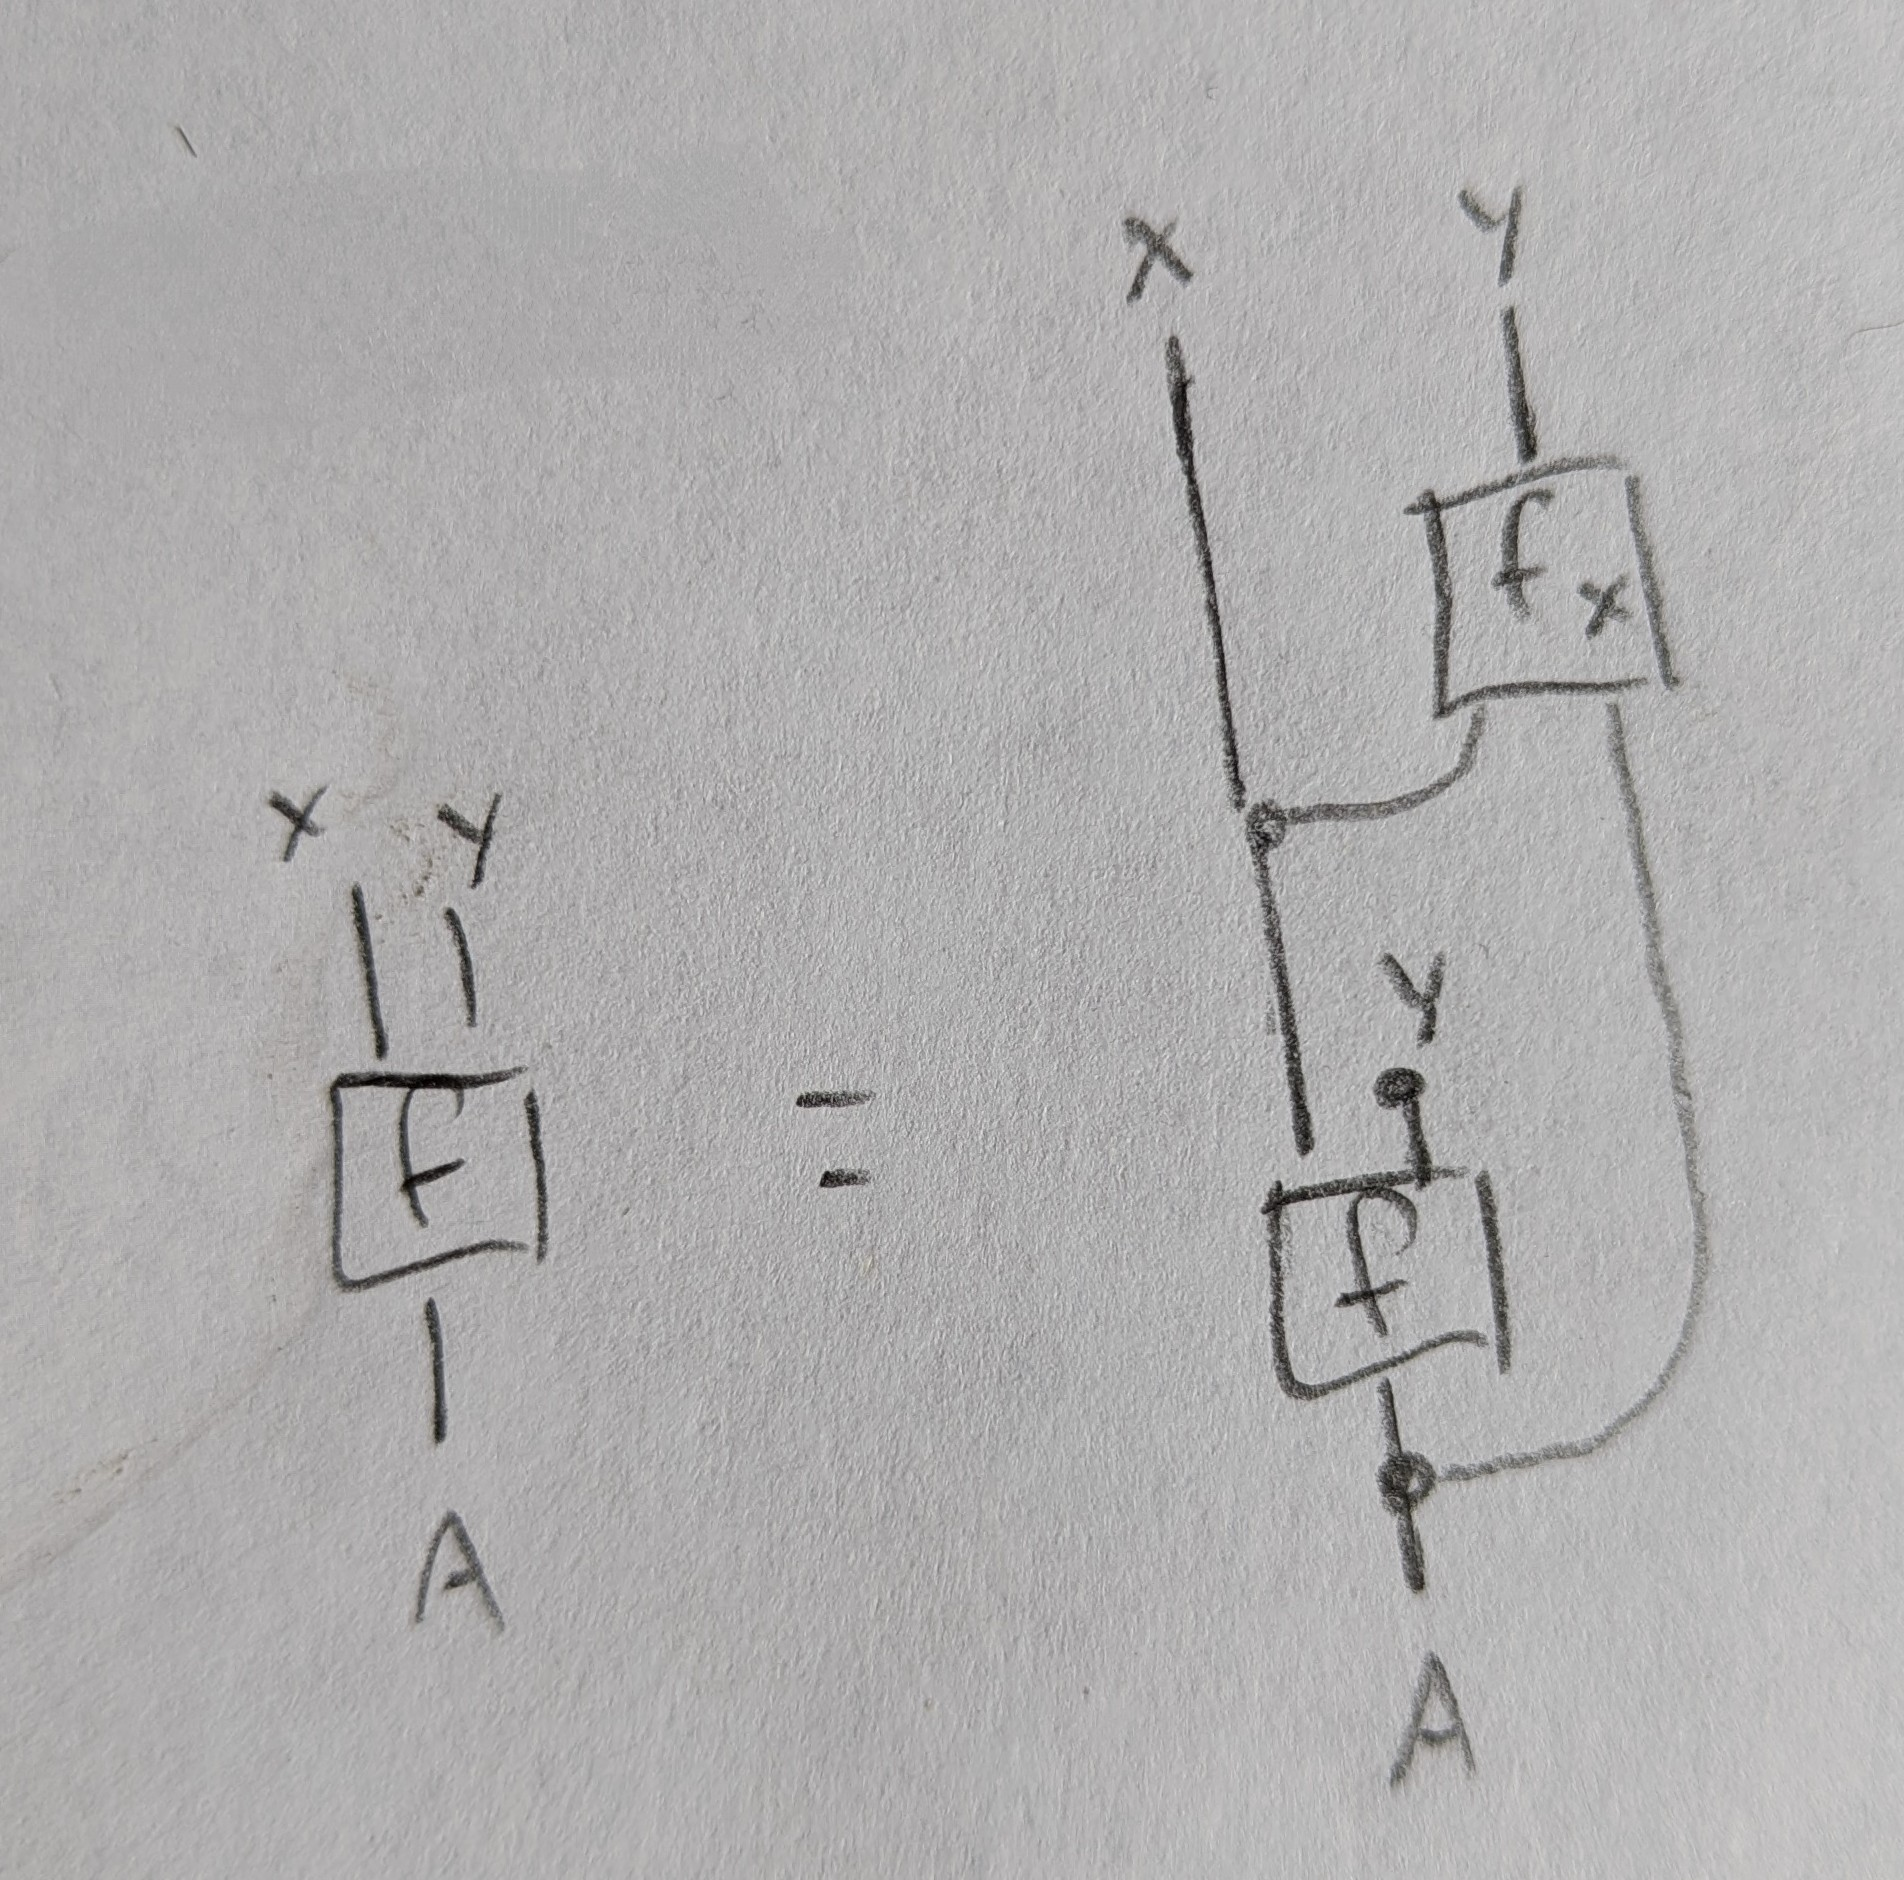
\includegraphics[width=0.5\textwidth]{conditional}
	\caption{The string diagram equation for the definition of conditioning.}
	\label{fig:conditional}
\end{figure}

\begin{figure}[htb]
	\centering
	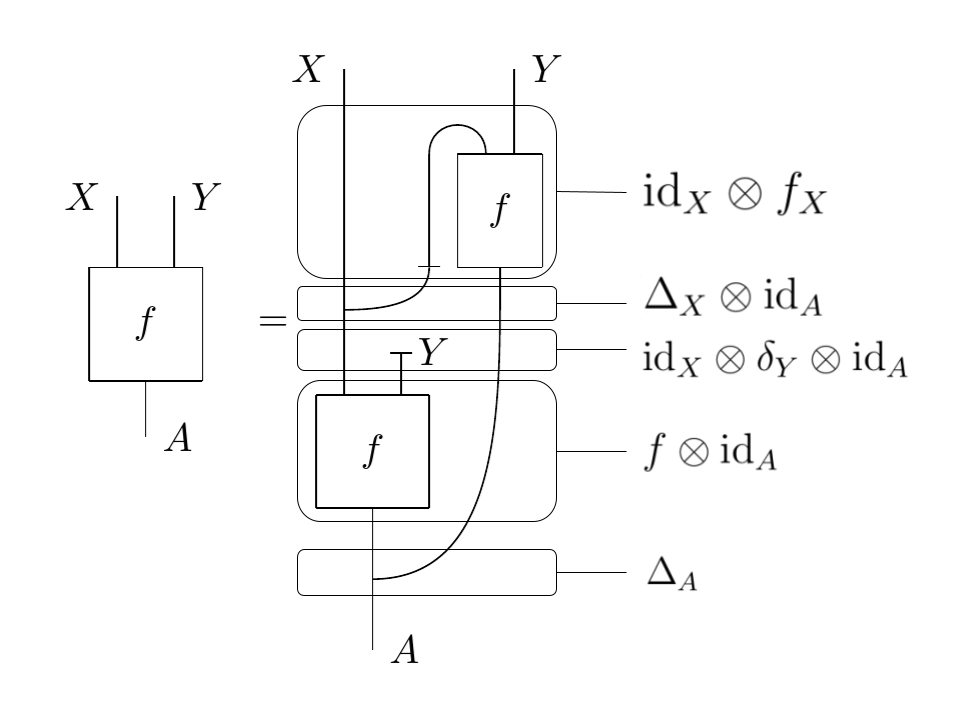
\includegraphics[width=0.5\textwidth]{conditional-compositions}
	\caption{The conditional equation is read like so. This corresponds to Equation \ref{eq:conditional-compositions}.}
	\label{fig:conditional-compositions}
\end{figure}

\begin{figure}[htb]
	\centering
	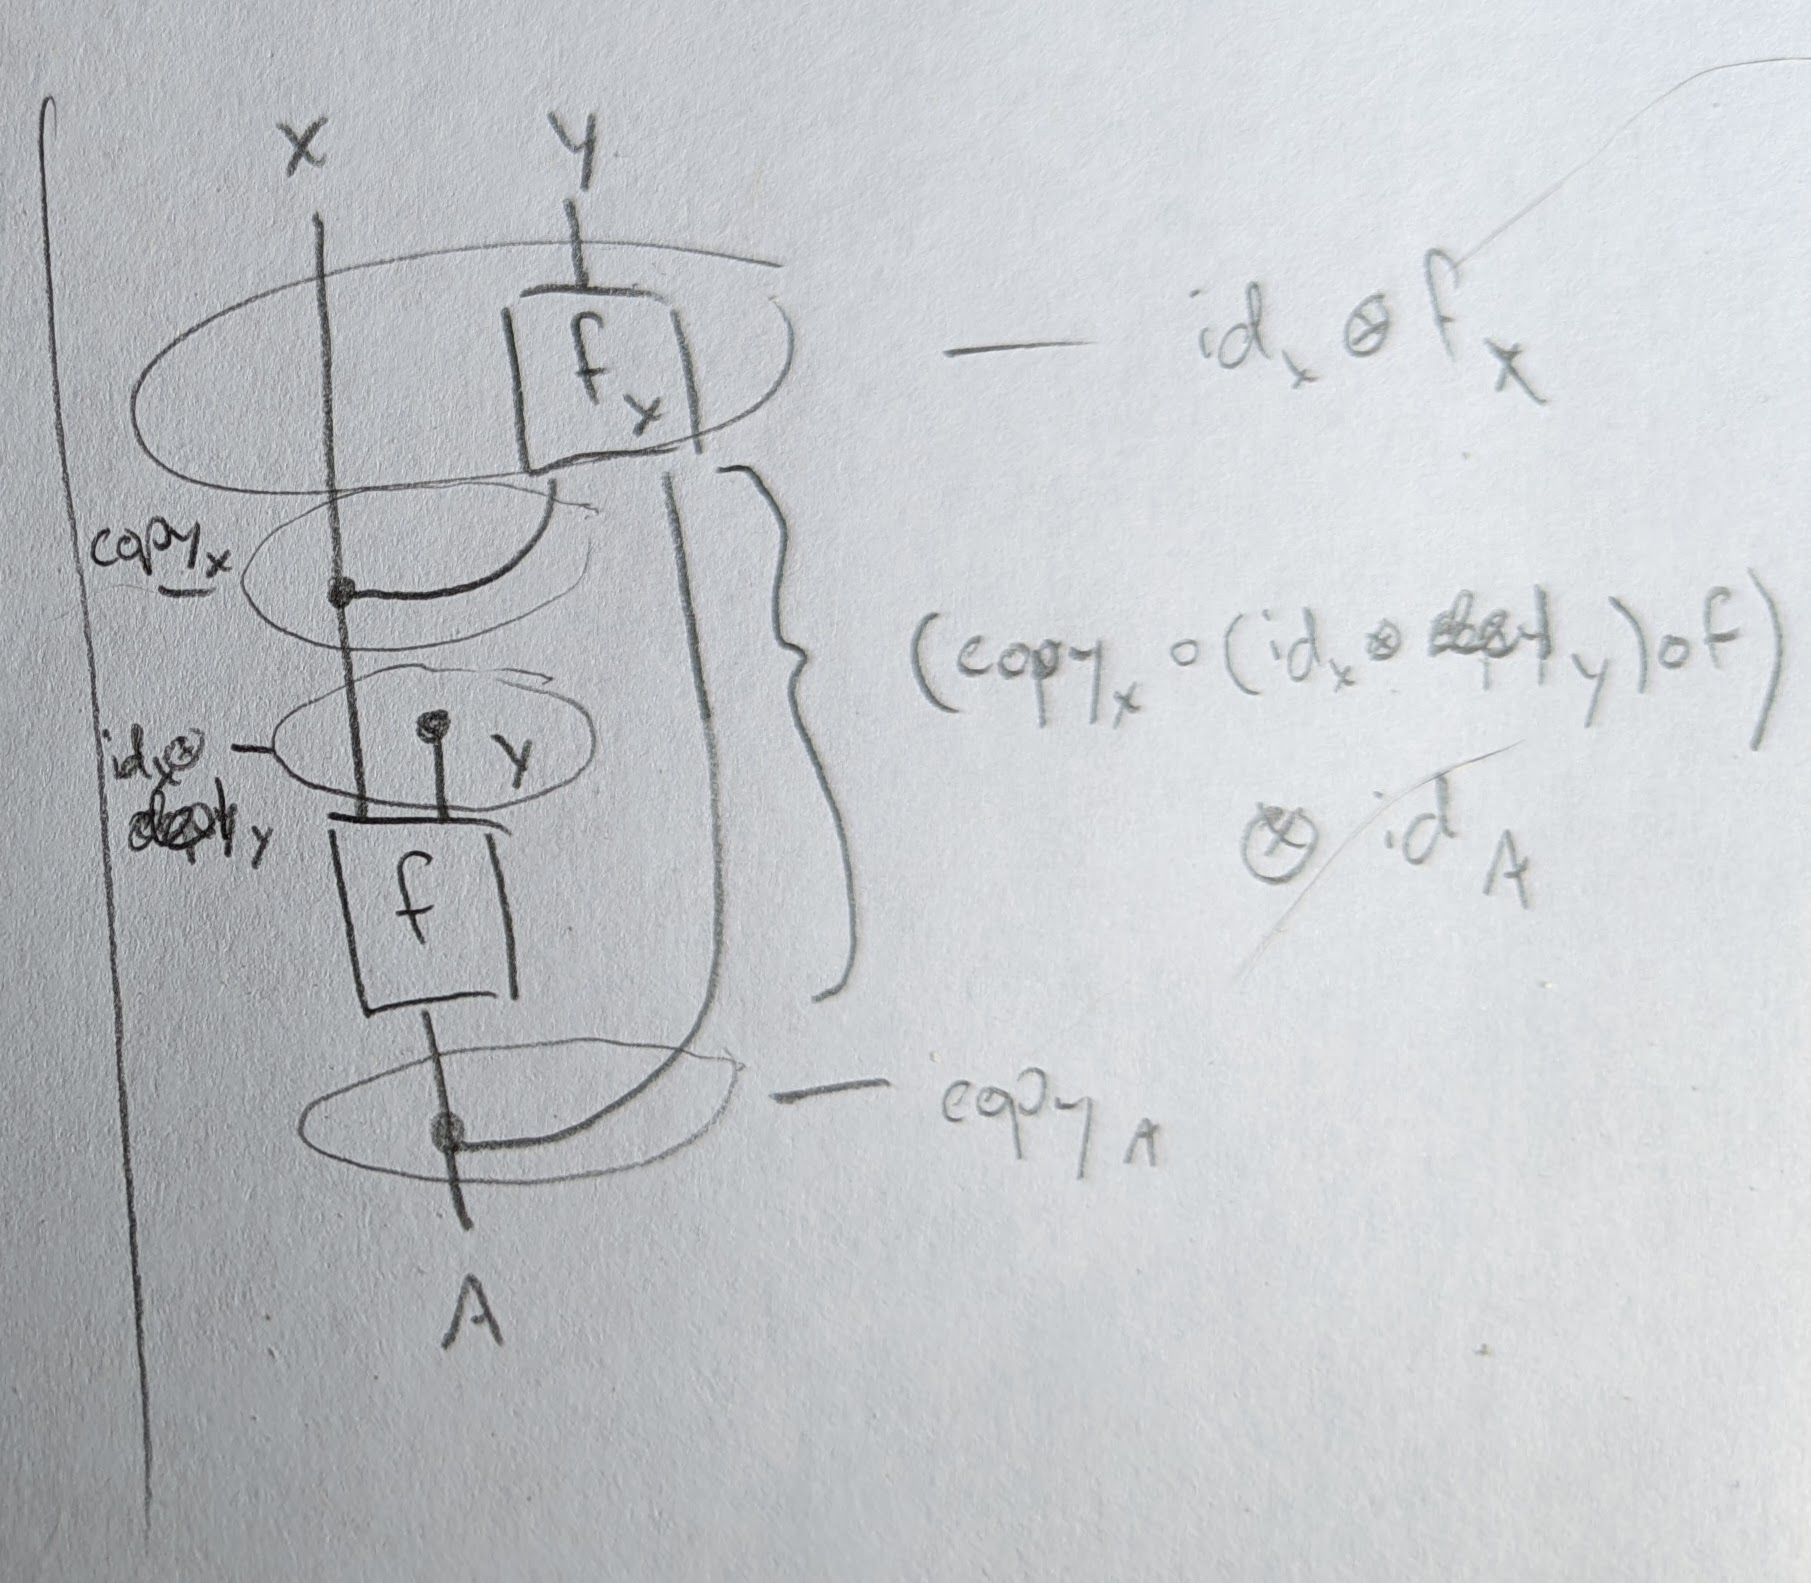
\includegraphics[width=0.5\textwidth]{conditional-parallel-compositions}
	\caption{The conditional equation can also be read this way. This corresponds to Equation \ref{eq:conditional-parallel-compositions}.}
	\label{fig:conditional-parallel-compositions}
\end{figure}

\begin{equation}
\label{eq:conditional-compositions}
f = (\counit_X \otimes f) \circ (\comul_X \otimes \id_A)
\circ (\id_X \otimes \counit_Y \otimes \id_A) \circ (f \otimes \id_A) \circ \comul_A
\end{equation}

\begin{equation}
\label{eq:conditional-parallel-compositions}
f = (\id_x \otimes f_x) \circ \left[\left(\comul_x \circ (\id_x\otimes \counit_Y) \circ f\right) \otimes \id_A\right] \circ \comul_A
\end{equation}

\section{Bar Notation}
\subsection{Explanation of Bar Notation}
\subsection{Translating Bar Notation into String Diagrams}

\chapter{Common Representations of Information Recast into the Language of Markov Categories}
\section{Discrete Probability}
\section{Gaussian Probability}
\section{Gaussian Mixtures: A Composition of Discrete and Gaussian Probability}
\section{Unscented Transform}

\chapter{Programming with Markov Categories}
\section{Making Datatypes}
\subsection{Gaussian}
\subsection{Unscented}
\subsection{Gaussian Mixtures}

\section{Synthetic Algorithms Used in Estimation and Control}
\subsection{Filtering}
\subsection{History Space}

